\documentclass[xcolor=dvipsnames]{beamer}
\usepackage{xcolor}
\usepackage{graphicx}


\usetheme{Antibes}
\usecolortheme{wolverine}

\setbeamercolor{emph}{fg=orange}
\renewcommand<>{\emph}[1]{%
  {\usebeamercolor[fg]{emph}\only#2{\itshape}#1}%
}

\title{Product Structure Theorems}
\author{Pat Morin}
\date{}
\institute{Carleton University \\[1em]
  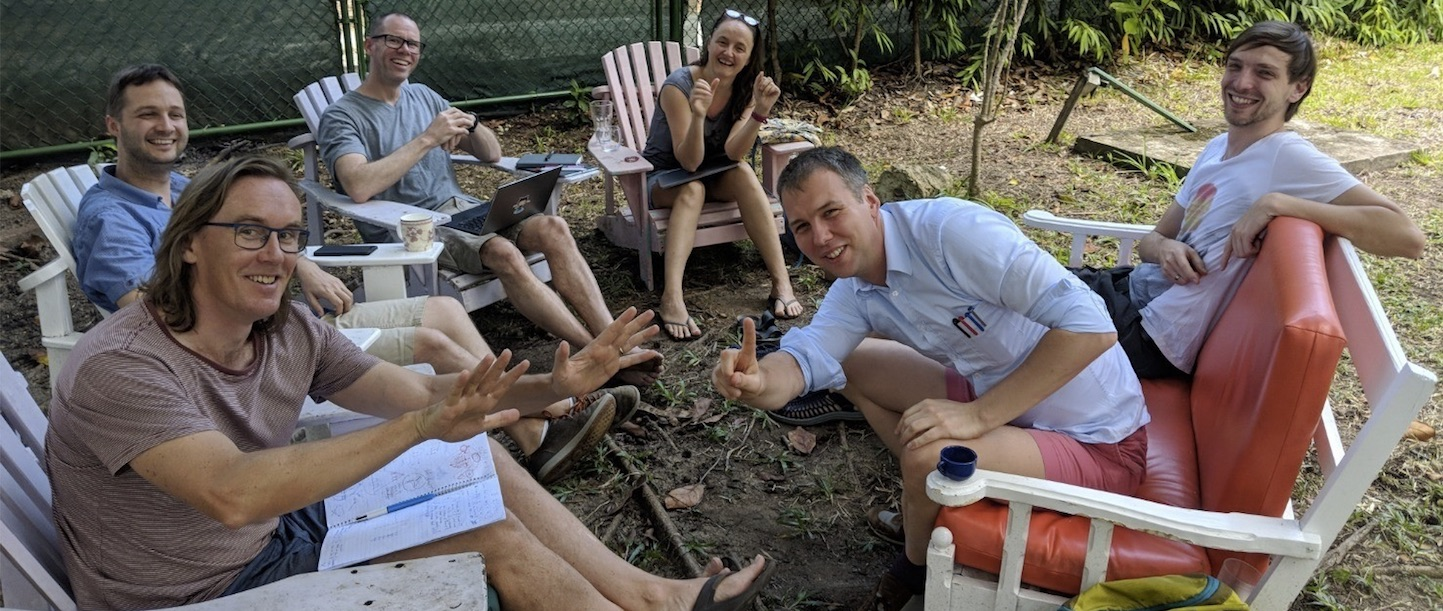
\includegraphics[width=.6\textwidth]{images/Queue11}
}


\newcommand{\colored}[2]{{\color{#1}#2}}


\begin{document}
\maketitle

\begin{frame}
  \frametitle{Outline}

  \begin{itemize}
    \item Motivation
    \item The Product Structure Theorem for planar graphs
    \item Proof sketch
    \item Generalizations
    \item Applications
  \end{itemize}
\end{frame}

\begin{frame}
  \frametitle{Ranking Graph Classes by Complexity}

  \colored{ForestGreen}{Simple}
  \begin{itemize}
    \item Paths (forests of paths)
    \item Trees (forests)
    \item $k$-Trees (graphs of treewidth at most $k$)
    \item $\vdots$
    \item Planar graphs
    \item $\vdots$
    \item All graphs
  \end{itemize}
  \colored{red}{Complicated}

  % \includegraphics{figs/product-lhs}
  % \includegraphics[scale=.5]{figs/planar-subgraph} \raisebox{.11\textwidth}{$\subseteq$}%
  % \only<1>{\includegraphics{figs/product-rhs}}%

\end{frame}


\begin{frame}
  \frametitle{Informally}

  \begin{itemize}[<+->]
    \item Can we \emph{factor} a planar graph into simpler graphs?
    \item Yes, every planar graph is contained in the \emph{strong product} of a graph $H$ of treewidth at most $8$ and a path $P$ \\
  \end{itemize}
  \includegraphics{figs/planar-subgraph}%
  \only<4>{\raisebox{.11\textwidth}{$\subseteq$}\includegraphics{figs/product-rhs}}%
  \only<3>{\raisebox{.11\textwidth}{$\subseteq$}\includegraphics{figs/product-lhs}}
\end{frame}


\begin{frame}
  \frametitle{The Strong Graph Product $\boxtimes$}
  \begin{itemize}
      \item[] For two graphs $A$ and $B$, the \emph{strong product} $A\boxtimes B$ is a graph:
      \begin{itemize}
          \item $V(A\boxtimes B):=V(A)\times V(B)$
          \item $(a_1,b_1)$ and $(a_2,b_2)$ are adjacent if and only if:
          \begin{itemize}
              \item $a_1=a_2$ and $b_1b_2\in E(B)$;
              \item $a_1a_2 \in E(A)$ and $b_1=b_2$; or
              \item  $a_1a_2 \in E(A)$ and $b_1b_2 \in E(B)$.
          \end{itemize}
      \end{itemize}
  \end{itemize}
  \begin{center}
      \includegraphics{figs/product-lhs} \raisebox{.11\textwidth}{$=$} \includegraphics{figs/product-rhs}
  \end{center}
\end{frame}

\begin{frame}
  \frametitle{The Product Structure Theorem for Planar Graphs}

  \textbf{Theorem (Dujmović-Joret-Micek-M-Ueckerdt-Wood 2019):} For every planar graph $G$, there exists a planar graph $H$ of treewidth at most $8$ and a path $P$ such that $G$ is a subgraph of $H\boxtimes P$.

  \includegraphics{figs/planar-subgraph}%
  % \only<4>{\raisebox{.11\textwidth}{$\subseteq$}\includegraphics{figs/product-rhs}}%
  \raisebox{.11\textwidth}{$\subseteq$}\includegraphics{figs/product-lhs}
\end{frame}

\begin{frame}
  \frametitle{Why?}

  $G\subseteq H\boxtimes P$
  \begin{itemize}[<+->]
    \item $H$ is a graph of treewidth at most $8$
    \item Many problems are easy for $H$
    \item Extending a solution from $H$ to $H\boxtimes P$ is sometimes easy
    \item Examples:
    \begin{itemize}
      \item queue number
      \item nonrepetitive colouring
      \item $p$-centered colouring
      \item $\ell$-vertex ranking
      \item Adjacency labelling (universal graphs)
    \end{itemize}
  \end{itemize}
  \begin{center}
    \resizebox{.5\textwidth}{!}{
      \includegraphics{figs/planar-subgraph}%
      \raisebox{.11\textwidth}{$\subseteq$}\includegraphics{figs/product-lhs}
    }
  \end{center}
\end{frame}

\begin{frame}
  \frametitle{The Precursor}

  \textbf{Theorem (Siebertz-Pilipczuk 201X):}  For any planar triangulation $G$, there exists a partition $\mathcal{P}$ of $V(G)$ such that
  \begin{itemize}
    \item<2-> Each part of $P$ induces a geodesic in $G$; and
    \item<3-> The quotient graph $H:=G/\mathcal{P}$ has treewidth at most $8$
  \end{itemize}

  \begin{center}
    \only<1>{\includegraphics[width=.8\textwidth]{figs/lhp-1}}%
    \only<2>{\includegraphics[width=.8\textwidth]{figs/lhp-2}}%
    \only<3->{\includegraphics[width=.8\textwidth]{figs/lhp-3}}%
    % \only<4->{\includegraphics[width=.8\textwidth]{figs/lhp-4}}%
    % \only<5>{\includegraphics{figs/lhp-5}}%
  \end{center}
\end{frame}

\begin{frame}
  \frametitle{Layered Partitions}
  \onslide<+->{
  \textbf{Theorem (Dujmović-Joret-Micek-M-Ueckerdt-Wood 2019):} For any planar triangulation $G$ and any breadth-first spanning-tree $T$ of $G$, there exists a partition $\mathcal{P}$ of $V(G)$ such that
  \begin{itemize}[<+->]
    \item Each part of $P$ induces a vertical path in $T$
    \item The quotient graph $H:=G/\mathcal{P}$ has treewidth at most $8$
  \end{itemize}
  }
  \begin{center}
    \only<1>{\includegraphics[width=.8\textwidth]{figs/lhp-4}}%
    \only<2>{\includegraphics[width=.8\textwidth]{figs/lhp-5}}%
    \only<3->{\includegraphics[width=.8\textwidth]{figs/lhp-6}}%
    % \only<4->{\includegraphics[width=.8\textwidth]{figs/lhp-4}}%
    % \only<5>{\includegraphics{figs/lhp-5}}%
  \end{center}
\end{frame}

\end{document}
